%
% This is a borrowed LaTeX template file for lecture notes for CS267,
% Applications of Parallel Computing, UCBerkeley EECS Department.
%

\documentclass{article}
\usepackage{titlesec}
%\setlength{\oddsidemargin}{0.25 in}
%\setlength{\evensidemargin}{-0.25 in}
\setlength{\oddsidemargin}{0 in}
\setlength{\evensidemargin}{0 in}
\setlength{\topmargin}{-0.6 in}
\setlength{\textwidth}{6.5 in}
\setlength{\textheight}{8.5 in}
\setlength{\headsep}{0.75 in}
\setlength{\parindent}{0 in}
\setlength{\parskip}{0.1 in}


%
% ADD PACKAGES here:
%

\usepackage{amssymb}	% Already loads amsfonts
\usepackage{amsthm}
\usepackage{graphicx}
\usepackage{mathtools}	% Already loads amsmath
\usepackage{hyperref}
\usepackage{enumitem}
\usepackage{clrscode3e}  % for typesetting pseudocode
\usepackage{ulem}
\usepackage[usenames,dvipsnames]{xcolor}
\usepackage{multicol}


% Tikz and setup
\usepackage{tikz}
\usepackage{tikz-cd}
\usetikzlibrary{intersections, angles, quotes, calc, positioning}
\usetikzlibrary{arrows.meta}
\usepackage{pgfplots}
\pgfplotsset{compat=1.13}


\tikzset{
    force/.style={thick, {Circle[length=2pt]}-stealth, shorten <=-1pt}
}

%
% The following commands set up the lecnum (lecture number)
% counter and make various numbering schemes work relative
% to the lecture number.
%
\newcounter{lecnum}
\renewcommand{\thepage}{\thelecnum-\arabic{page}}
\renewcommand{\thesection}{\thelecnum.\arabic{section}}
\renewcommand{\theequation}{\thelecnum.\arabic{equation}}
\renewcommand{\thefigure}{\thelecnum.\arabic{figure}}
\renewcommand{\thetable}{\thelecnum.\arabic{table}}

%
% The following macro is used to generate the header.
%
\newcommand{\lecture}[5]{
   \pagestyle{myheadings}
   \thispagestyle{plain}
   \newpage
   \setcounter{lecnum}{#2}
   \setcounter{page}{1}
   \noindent
   \begin{center}
   \framebox{
      \vbox{\vspace{2mm}
    \hbox to 6.28in { {\bf #1
	\hfill} }
       \vspace{4mm}
       \hbox to 6.28in { {\Large \hfill Lecture #2: #3  \hfill} }
       \vspace{2mm}
       \hbox to 6.28in { {\it Lecturer: #4 \hfill Scribe: #5} }
      \vspace{2mm}}
   }
   \end{center}
   \markboth{Lecture #2: #3}{Lecture #2: #3}
   \vspace*{4mm}
}
\renewcommand{\cite}[1]{[#1]}
\def\beginrefs{\begin{list}%
        {[\arabic{equation}]}{\usecounter{equation}
         \setlength{\leftmargin}{2.0truecm}\setlength{\labelsep}{0.4truecm}%
         \setlength{\labelwidth}{1.6truecm}}}
\def\endrefs{\end{list}}
\def\bibentry#1{\item[\hbox{[#1]}]}

\newcommand{\fig}[3]{
			\vspace{#2}
			\begin{center}
			Figure \thelecnum.#1:~#3
			\end{center}
	}

% Colored theorem styles
\makeatother
\usepackage{thmtools}
\usepackage[framemethod=TikZ]{mdframed}
\mdfsetup{skipabove=1em,skipbelow=1em}

\declaretheoremstyle[
    headfont=\bfseries\sffamily\color{ForestGreen!70!black}, bodyfont=\normalfont,
    mdframed={
        linewidth=2pt,
        rightline=false, topline=false, bottomline=false,
        linecolor=ForestGreen, backgroundcolor=ForestGreen!5,
    },
    spaceabove=8pt
]{thmgreenbox}

\declaretheoremstyle[
    headfont=\bfseries\sffamily\color{NavyBlue!70!black}, bodyfont=\normalfont,
    mdframed={
        linewidth=2pt,
        rightline=false, topline=false, bottomline=false,
        linecolor=NavyBlue, backgroundcolor=NavyBlue!5,
    },
    spaceabove=8pt
]{thmbluebox}

\declaretheoremstyle[
    headfont=\bfseries\sffamily\color{NavyBlue!70!black}, bodyfont=\normalfont,
    mdframed={
        linewidth=2pt,
        rightline=false, topline=false, bottomline=false,
        linecolor=NavyBlue
    },
    spaceabove=8pt
]{thmblueline}

\declaretheoremstyle[
    headfont=\bfseries\sffamily\color{RawSienna!70!black}, bodyfont=\normalfont,
    mdframed={
        linewidth=2pt,
        rightline=false, topline=false, bottomline=false,
        linecolor=RawSienna, backgroundcolor=RawSienna!5,
    },
    spaceabove=8pt
]{thmredbox}

\declaretheoremstyle[
    headfont=\bfseries\sffamily\color{RawSienna!70!black}, bodyfont=\normalfont,
    numbered=no,
    mdframed={
        linewidth=2pt,
        rightline=false, topline=false, bottomline=false,
        linecolor=RawSienna, backgroundcolor=RawSienna!1,
    },
    qed=\qedsymbol,
    spaceabove=8pt
]{thmproofbox}

\declaretheoremstyle[
    headfont=\bfseries\sffamily\color{NavyBlue!70!black}, bodyfont=\normalfont,
    numbered=no,
    mdframed={
        linewidth=2pt,
        rightline=false, topline=false, bottomline=false,
        linecolor=NavyBlue, backgroundcolor=NavyBlue!1,
    },
    spaceabove=8pt
]{thmexplanationbox}

% Use these for theorems, lemmas, proofs, etc.
\theoremstyle{definition}
\declaretheorem[style=thmgreenbox, name=Definition, numberwithin=lecnum]{definition}
\declaretheorem[style=thmbluebox, numbered=no, name=Example]{example}
\declaretheorem[style=thmredbox, name=Theorem, numberwithin=lecnum]{theorem}
\declaretheorem[style=thmredbox, name=Proposition, sibling=theorem]{proposition}
\declaretheorem[style=thmredbox, name=Lemma, sibling=theorem]{lemma}
\declaretheorem[style=thmredbox, name=Corollary, sibling=theorem]{corollary}
% \newtheorem{theorem}{Theorem}[lecnum]
% \newtheorem{lemma}[theorem]{Lemma}
% \newtheorem{claim}[theorem]{Claim}
% \newtheorem{corollary}[theorem]{Corollary}
% \newtheorem{definition}[theorem]{Definition}
\declaretheorem[style=thmblueline, numbered=no, name=Remark]{remark}
\renewenvironment{proof}{{\bf \textit{Proof.}}}{\hfill\rule{2mm}{2mm}}
\makeatletter


% **** IF YOU WANT TO DEFINE ADDITIONAL MACROS FOR YOURSELF, PUT THEM HERE:

\renewcommand\Pr{\mathbb{P}}
\newcommand\Ex{\mathbb{E}}

\newcommand\N{\mathbb{N}}
\newcommand\Z{\mathbb{Z}}
\newcommand\Q{\mathbb{Q}}
\newcommand\R{\mathbb{R}}
\newcommand\C{\mathbb{C}}
\newcommand\F{\mathbb{F}}

\DeclarePairedDelimiter\ceil{\lceil}{\rceil}
\DeclarePairedDelimiter\floor{\lfloor}{\rfloor}
\DeclarePairedDelimiter\anglebrac{\langle}{\rangle}

\begin{document}
\lecture{MAT344 Intro to Combinatorics}{10}{Pr\"ufer Code and Counting Trees, Poset}{Keegan Dasilva Barbosa}{Kevin Gao}

\section{Counting Trees}

Recall that a tree is a connected graph with the property that any two vertices are connected by a unique path. Equivalently, a tree is a connected graph with $n-1$ edges and $n$ vertices. A tree with at least $n \geq 2$ vertices has at least two vertices of degree one (the leaves).

\begin{definition}[Labeled Tree]
    A \textit{\textbf{labeled tree}} is a tree $T$ whose vertex set is $\{1,\ldots,n\}$.
\end{definition}

We would like to know how many possible $E$ exist such that $([n], E)$ forms a \textbf{labeled tree}. We are not counting isomorphisms here so the labels matter. To answer this question, we introduce \textbf{Pr\"ufer's cod}e, which transforms trees into strings that are easy to count.

\subsection{Pr\"ufer Code}

Fix $n \geq 2$. Let $s:\; [n-2] \to \{1,\ldots,n\}$ be a sequence (string over $\{1,\ldots,n\}$ of length $n-1$). Consider the following algorithm that generates a set $E$ of size $n-2$.
\begin{codebox}
    \Procname{$\proc{Prufer-Decode}(s)$}
    \li $L = \{1,\ldots,n\}$
    \li \While $|s| > 0$ \Do
        \li find the smallest $j$ that is not in $s$, add $\{j,s[1]\}$ to $E$
        \li set $L = L \setminus \{j\}$
        \li delete $s[1]$
    \End
    \li set $E = E \cup \{L\}$
    \li \Return $E$
\end{codebox}
The algorithm above assigns to each sequence $s$, a set $E$ of size $n-1$ such that $([n], E)$ is connected.

\begin{figure}[htbp]
    \centering
    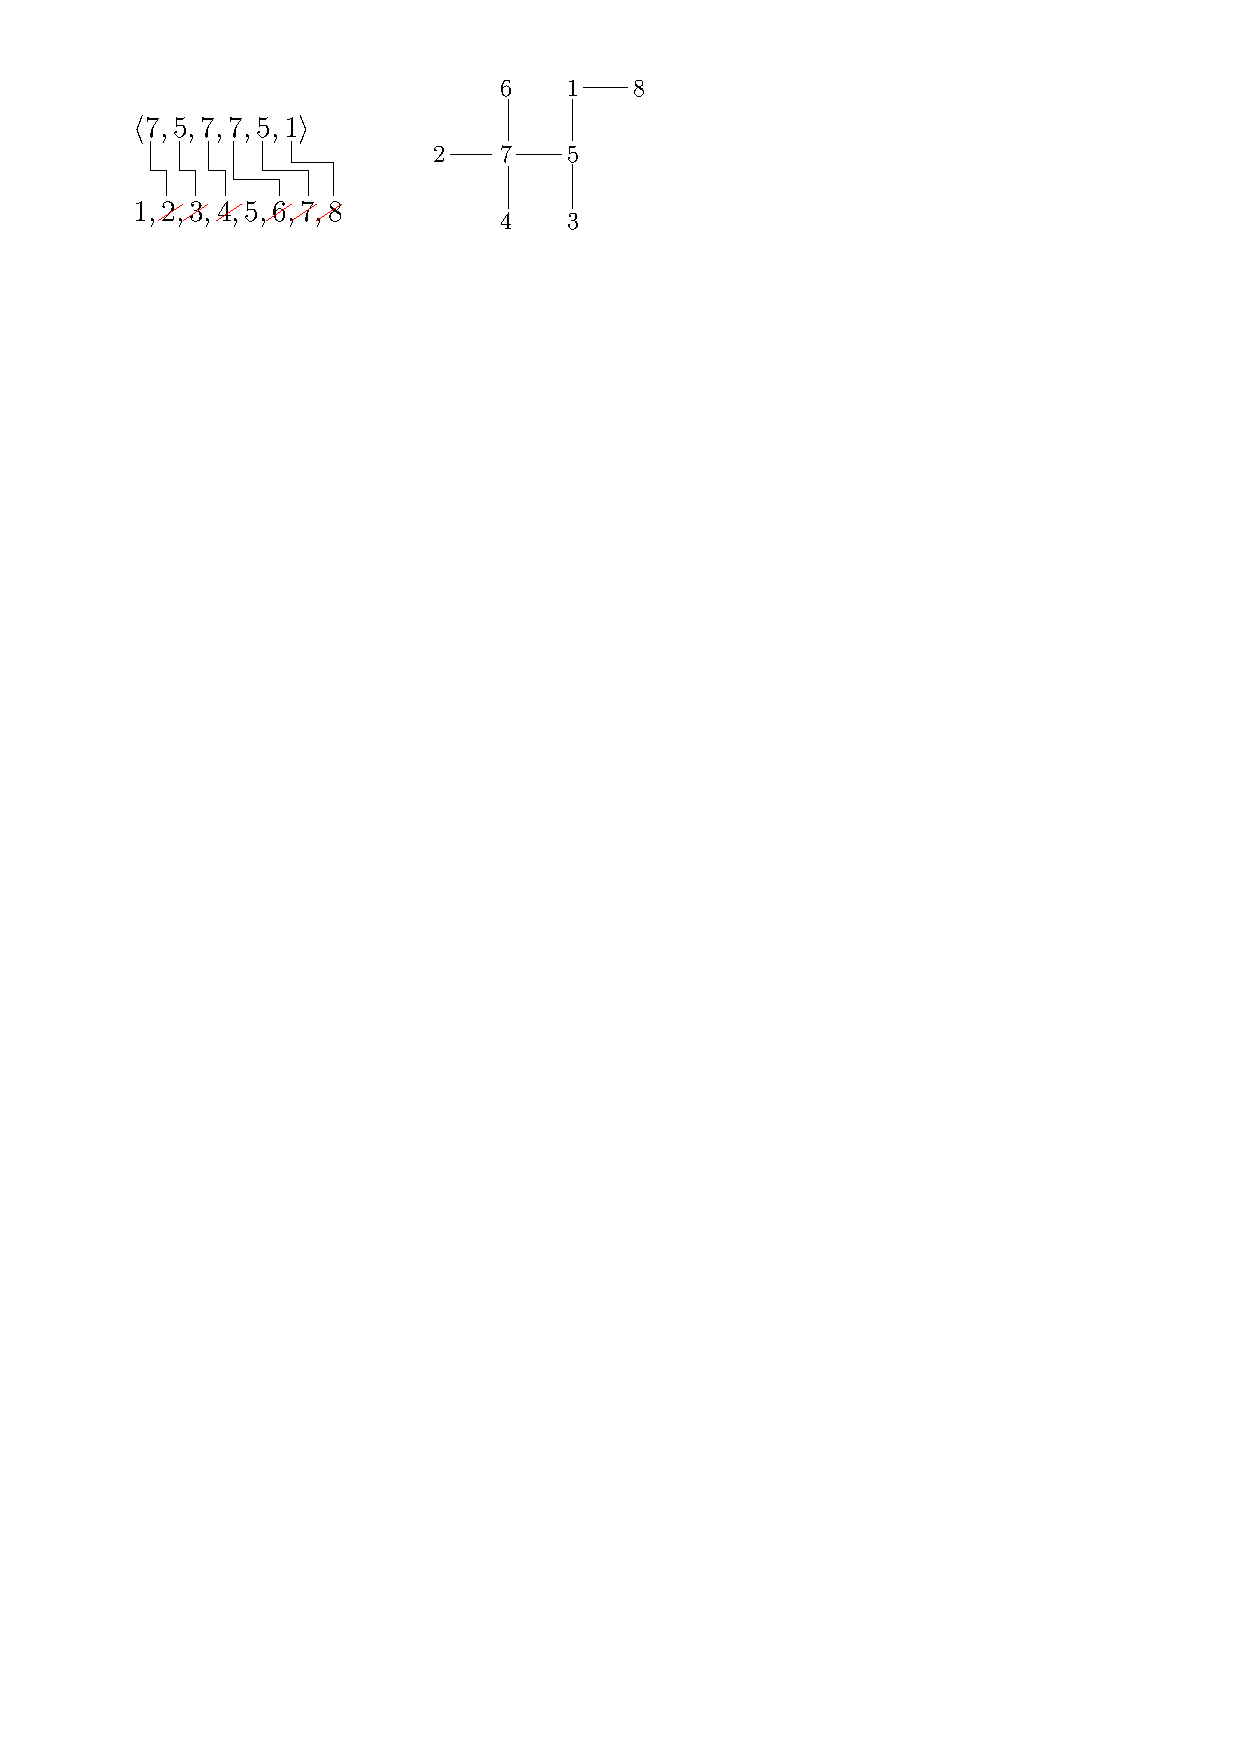
\includegraphics[width=0.5\linewidth]{figures/prufer-code-example.pdf}
    \caption{Example of a tree and its corresponding Prufer code}
    \label{fig:prufer-code-example}
\end{figure}

We can reverse the algorithm above to encode a tree into its Pr\"ufer code.

\begin{codebox}
    \Procname{$\proc{Prufer-Encode}(E)$}
    \li \For $i = 1$ \To $n-2$ \Do
        \li $s[i]$ = the unique vertex adjacent to the leaf with the smallest value
        \li remove the leaf with the smallest value
    \End
    \li \Return $s$
\end{codebox}

\subsection{Back to Counting Trees}

Each labeled tree with $n$ vertices has a unique Pr\"ufer's code of length $n-2$. Then, counting the number of labeled trees is equivalent to counting the number of Pr\"ufer codes for all the trees.

\begin{theorem}[Cayley's Formula]
    For each $n \geq 2$, there are exactly $n^{n-2}$ labeled trees on $\{1,\ldots,n\}$.
\end{theorem}

\begin{proof}
    To each tree, find the unique associated Pr\"ufer code $s:\; [n-2] \to [n]$. This creates a bijective correspondence between labeled trees and sequences $s:\; [n-2] \to [n]$.

    There are exactly $n^{n-2}$ such sequences and hence that many labeled trees on $\{1,\ldots,n\}$.
\end{proof}

\section{Poset}

\begin{definition}[Poset (partially ordered set)]
    A \textit{\textbf{poset}} $\mathbb{P}$ is a pair $\mathbb{P} = (X,P)$ where $X$ is a set and $P \subseteq X \times X$ is a relation that is
    \begin{itemize}
        \item reflexive: $\forall a \in X.\, (a,a) \in P$
        \item anti-symmetric: $a \neq b \land (a,b) \in P \implies (b,a) \not\in P$
        \item transitive: $(a,b) \in P \land (b,c) \in P \implies (a,c) \in P$
    \end{itemize}
\end{definition}

Instead of writing $(a,b) \in P$, we use the notation $a \leq_{\mathbb{P}} b$.

\begin{definition}[Embedding, Isomorphism, Automorphism]
    Given a poset $\mathbb{P} = (X,P)$ and $\mathbb{Q} = (Y,Q)$, an \textbf{embedding} from $\mathbb{P}$ into $\mathbb{Q}$ is an injective map $f:\; X \to Y$ with the property that $a \leq_{\mathbb{P}} b$ if and only if $f(a) \leq_{\mathbb{Q}} f(b)$. If the embedding is surjective, we call it an \textbf{isomorphism}. If $\mathbb{Q} = \mathbb{P}$, we call it an \textbf{automorphism}.
\end{definition}

For example, consider $X = \{\star, \circ, \diamond \}$ with $P = \{ (\star,\star), (\circ,\circ), (\diamond, \diamond), (\diamond, \star) \}$, and $Y = \{\star, \circ, \diamond, \Box \}$ with $Q = \{ (\star,\star), (\circ,\circ), (\diamond,\diamond), (\Box,\Box), (\Box,\star) \}$. Let $\mathbb{P} = (X,P)$ and $\mathbb{Q} = (Y,Q)$. Consider the function $f:\; X \to Y$ such that $f(\star) = \star$, $f(\circ) = \circ$, and $f(\diamond) = \Box$. $f$ is an embedding because $\diamond \leq_{\mathbb{P}} \star$ if and only if $f(\diamond) = \Box \leq_{\mathbb{Q}} \star = f(\star)$. However, $f$ is not an isomorphism because $\diamond$ is not in the range of $f$ so $f$ is not surjective.

\begin{definition}[Dual]
    Given a poset $\mathbb{P} = (X,P)$, we call the poset $\mathbb{P}^d = (X,P^d)$ where $a \leq_{\mathbb{P}^d} b \iff b \leq_{\mathbb{P}_d} a$ the \textbf{dual} of $\mathbb{P}$. We say a poset is self-dual if it is isomorphic to its dual.
\end{definition}

\begin{definition}[Cover]
    Given a poset $\mathbb{P} = (X,P)$ and a point $a \in X$, we say $a$ is \textbf{covered by} a point $b \in X$ if $a <_{\mathbb{P}} b$ and there is no $c$ such that $a <_{\mathbb{P}} c <_{\mathbb{P}} b$.
\end{definition}

\begin{definition}[Cover Graph]
    Given a poset $\mathbb{P} = (X,P)$, we call the graph $G = (X,E)$ given by $\{x,y\} \in E$ if and only if $x$ covers $y$ or $y$ covers $x$, the \textbf{cover graph} associated to $\mathbb{P}$. 
\end{definition}

If we draw the cover graph in an oriented fashion where lower vertices correspond to the $\leq_{\mathbb{P}}$-smaller elements, we have a special kind of cover graph known as \textbf{Hasse diagram}.

Let $\mathbb{P} = (X,P)$ be a poset where $X = \{a,b,c,d,e,f\}$ and $P = \{ (a,c), (b,c), (b,d), (d,e), (a,e), (e,f)\}$. One possible cover graph and the Hasse diagram is shown below.

\begin{figure}[htbp]
    \centering
    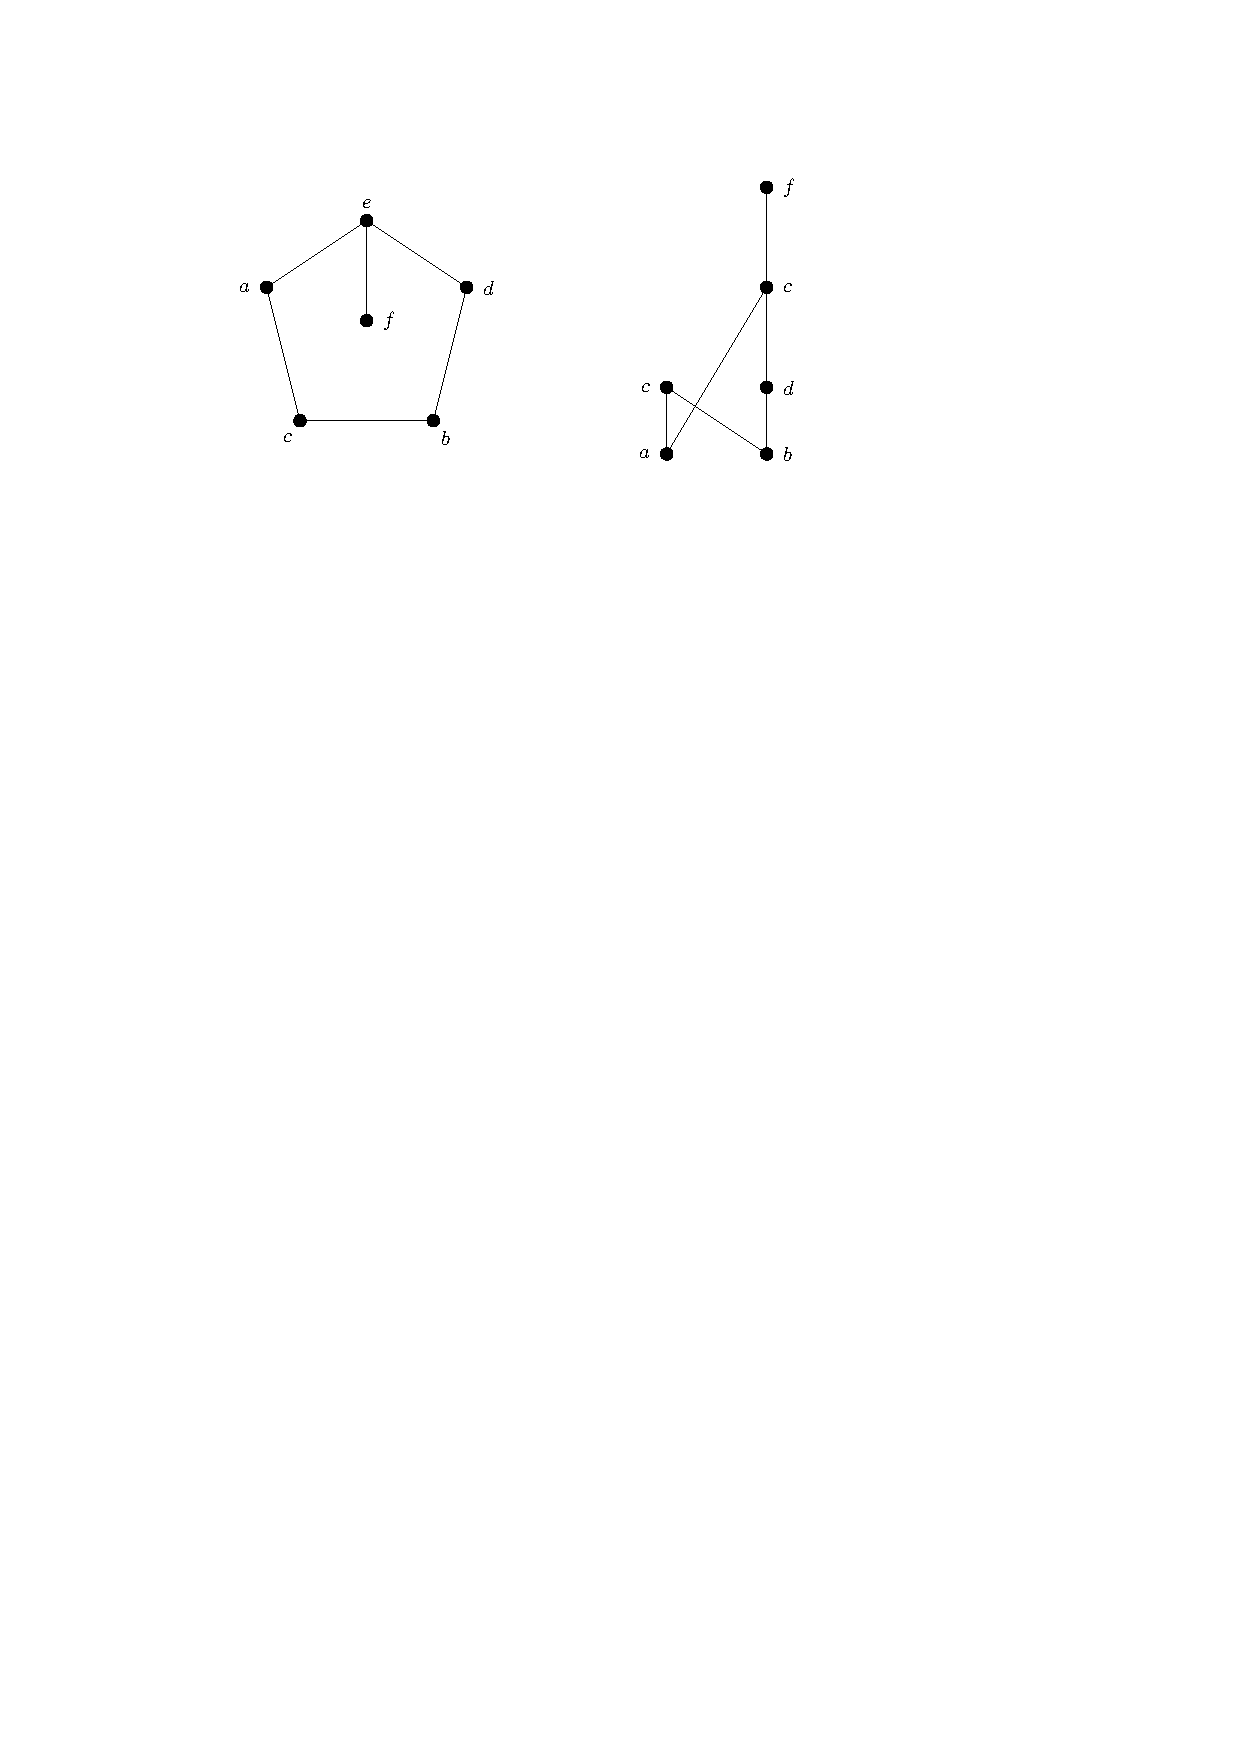
\includegraphics[width=0.5\linewidth]{figures/hasse-diagram.pdf}
    \caption{Cover graph and Hasse diagram for the poset described above.}
    \label{fig:hasse-diagram-example}
\end{figure}

\subsection{Linear Orders}

\begin{definition}[Comparability]
    Given a poset $\mathbb{P} = (X,P)$, we say two points $a,b \in X$ are \textit{\textbf{comparable}} if either $a <_{\mathbb{P}} b$ or $b <_{\mathbb{P}} b$ If two points are not comparable, we call them \textit{\textbf{incomparable}}.
\end{definition}

\begin{definition}[Total/Linear Order]
    Given a poset $\mathbb{P} = (X,P)$, we say $\mathbb{P}$ is \textit{\textbf{linearly ordered}} or \textit{\textbf{totally ordered}} if no two distinct points are incomparable.
\end{definition}

\subsection{Height and Width}

\begin{definition}[Antichain and Chain]
    Given a poset $\mathbb{P} = (X,P)$, we call $A \subseteq X$ an \textit{\textbf{antichain}} if every pair of distinct elements in $A$ are \textbf{incomparable}. We call a subset $C \subseteq X$ a \textit{\textbf{chain}} is every pair of distinct elements is \textbf{comparable}.
\end{definition}

\begin{definition}[Height and Width]
    Given a poset $\mathbb{P} = (X,P)$, we define the parameters $\mathsf{width}(\mathbb{P})$ and $\mathsf{height}(\mathbb{P})$ to denote the size of the largest antichain and chain of $\mathbb{P}$, respectively.
\end{definition}

\subsection{Subset Lattice and Sperner's Theorem}

\begin{theorem}[Sperner's Theorem]
    Consider the poset $\mathbb{P} = (\mathcal{P}([n]), \subseteq)$. Then, $\mathsf{width}(\mathbb{P}) = \binom{n}{\floor{n/2}}$.
\end{theorem}

\begin{proof}
    One can easily verify that $A = \{ S \subseteq [n] \mid |S| = \floor{\frac{n}{2}}\}$ is an \textbf{antichain}. Two sets of the same size are comparable if and only if they are equal. There are $\binom{n}{\floor{\frac{n}{2}}}$ such subsets of $[n]$ of size $\floor{\frac{n}{2}}$, so $\mathsf{width}(\mathbb{P}) \geq \binom{n}{\floor{\frac{n}{2}}}$. This shows that $\binom{n}{\floor{\frac{n}{2}}}$ is a lower bound.

    Now, we proceed to show that $\binom{n}{\floor{\frac{n}{2}}}$ is also an upper bound. Let $A = \{ S_1, \ldots, S_w \}$ be a \textbf{maximal antichain} of $\mathbb{P}$. It suffices to show that $w \leq \binom{n}{\floor{\frac{n}{2}}}$. For each $S_i \in A$, let $\mathcal{C}_i$ be the set of all \textbf{maximal chains} that contains $S_i$. We note that a maximal chain but be an $\subseteq$-increasing sequences that differs by at most one element per successive cover. If the next subset in the chain \textbf{differs} from the previous subset \textbf{by more than one element}, then the chain \textbf{would not be maximal}. In other words, starting from $S_i$, we remove 1 element until we reaches the empty set, and add 1 element until we reaches $[n]$. There are $|S_i|!$ ways to remove points successively from $S_i$. Similarly, there are $(k-|S_i|)!$ ways to add points successively to $S_i$. Therefore, for any $i$, $|\mathcal{C}_i| = |S_i|! \cdot (k-|S_i|)!$.

    \begin{figure}[htbp]
        \centering
        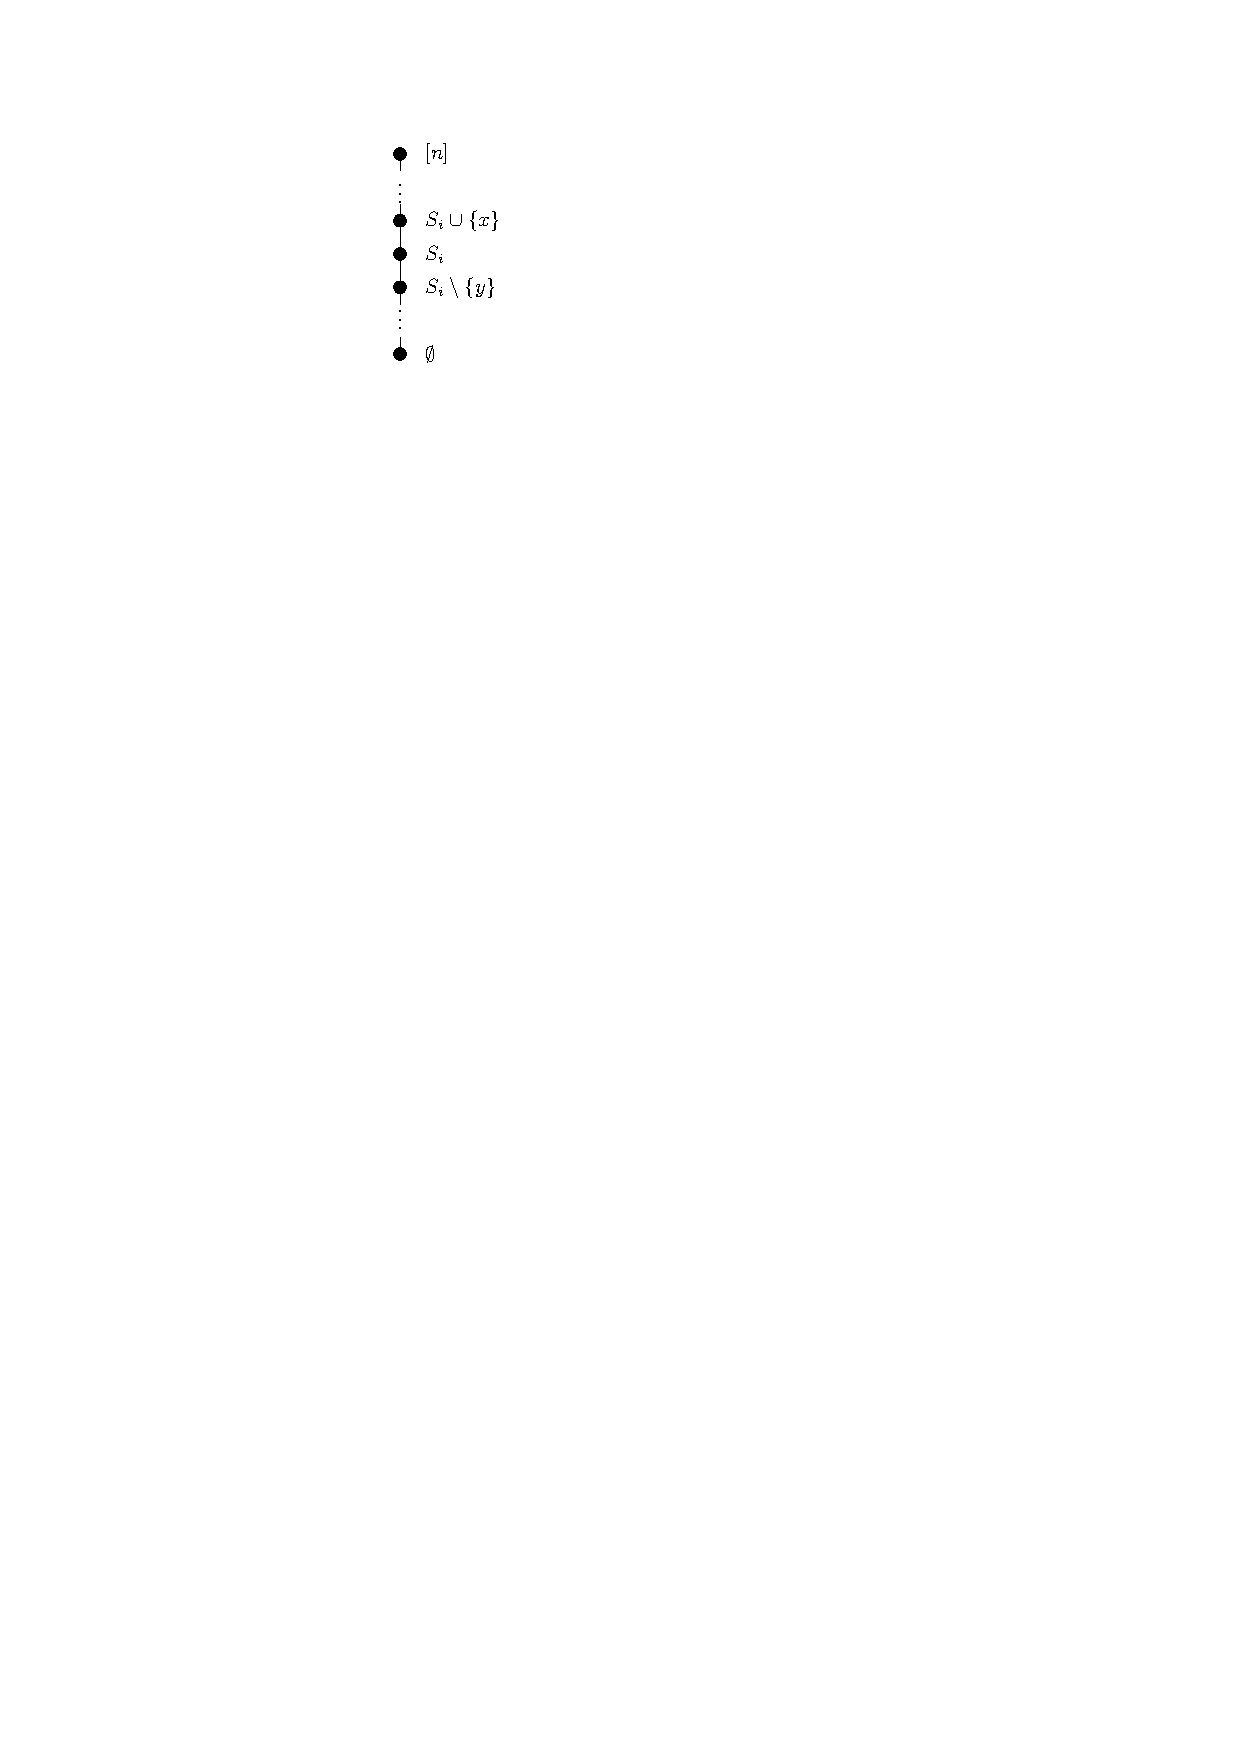
\includegraphics[width=0.1\linewidth]{figures/max-len-chain.pdf}
        \caption{Each subset must differ from the previous and next subset by exactly one element in a maximal chain. Otherwise, we form a chain of longer length by inserting a new subset in between.}
        \label{fig:max-len-chain}
    \end{figure}

    We also observe that there are exactly $n!$ many maximal chains, each corresponding to one ordering (permutation) to remove elements from $[n]$.

    For any $i \neq j$, $\mathcal{C}_i \cap \mathcal{C}_j = \emptyset$ because otherwise there would be a chain $C$ with $S_i,S_j \in C$ and hence $S_i$ and $S_j$ are comparable, which is a contradiction to our assumption that $S_i$ and $S_j$ are members of a maximal \textbf{antichain}. It follows that
    $$
    \left| \bigcup_{i=1}^w \mathcal{C}_i \right| = \sum_{i=1}^w |\mathcal{C}_i| \leq n!
    $$
    Since $|\mathcal{C}_i| = |S_i|! \cdot (k-|S_i|)!$, it follows that
    $$
    \sum_{i=1}^w |\mathcal{C}_i| = \sum_{i=1}^w (|S_i|! \cdot (k-|S_i|)!) \leq n!
    $$
    and hence
    $$
    \sum_{i=1}^w \frac{|S_i|! \cdot (k-|S_i|)!}{n!} = \sum_{i=1}^w \frac{1}{\binom{n}{|S_i|}} \leq 1
    $$
    by definition of combination. It follows from $\binom{n}{|S_i|} \leq \binom{n}{\floor{n/2}}$ that
    $$
    \sum_{i=1}^w \frac{1}{\binom{n}{\floor{n/2}}} \leq \sum_{i=1}^w \frac{1}{\binom{n}{|S_i|}}\leq 1
    $$
    and $w \leq \binom{n}{\floor{\frac{n}{2}}}$. Therefore, $\mathsf{width}(\mathbb{P}) \leq \binom{n}{\floor{\frac{n}{2}}}$ and because $\binom{n}{\floor{\frac{n}{2}}}$ is also a lower bound, $\mathsf{width}(\mathbb{P}) = \binom{n}{\floor{\frac{n}{2}}}$.
\end{proof}

\end{document}